\documentclass[10pt,a4paper]{article}
\usepackage[a4paper,margin=1.6cm,top=1.3cm,bottom=1.4cm]{geometry}
\usepackage[T1]{fontenc}
\usepackage[utf8]{inputenc}
\usepackage{lmodern}
\usepackage{microtype}
\usepackage{tikz}
\usetikzlibrary{positioning,fit,arrows.meta,backgrounds}
\usepackage{tabularx,booktabs,array}
\usepackage{enumitem}
\usepackage[hidelinks]{hyperref}
\usepackage{titlesec}

\pagestyle{empty}
\setlength{\parindent}{0pt}
\setlength{\parskip}{2pt}
\titleformat{\section}{\large\bfseries}{}{0pt}{}
\titlespacing*{\section}{0pt}{5pt}{2pt}
\setlist{nosep,leftmargin=*}
\newcommand{\cmp}[1]{\textbf{#1}}

\begin{document}

% ---------- Header (template fields) ----------
\begin{tabularx}{\textwidth}{@{}l X@{}}
\textbf{Project:} & Project 3 -- Cloud-Native Trade Anomaly Detection \& Reporting Platform (client: DNEXT) \\
\textbf{Group:} & 16 \\
\textbf{Students:} & Tania Nunez, Jeremiah Steiner, Aladin Iseni \\
\textbf{Link to a video:} & \textit{[to be added]} \\
\end{tabularx}

% ---------- Architecture ----------
\section*{Architecture}

\begin{center}
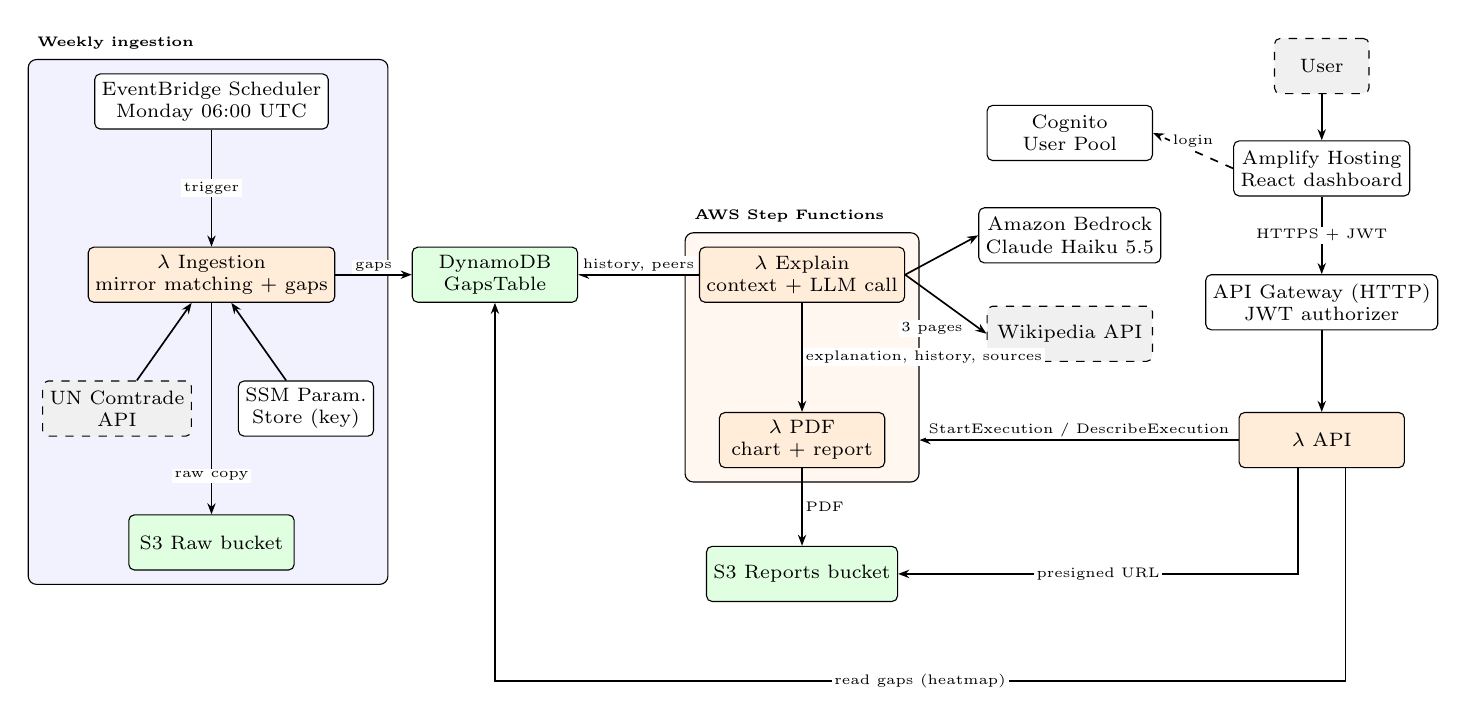
\begin{tikzpicture}[
  font=\scriptsize,
  box/.style={draw, rounded corners=2pt, fill=white, align=center, minimum height=0.7cm, minimum width=2.1cm, inner sep=2.5pt},
  lam/.style={box, fill=orange!15},
  sto/.style={box, fill=green!12},
  ext/.style={box, fill=gray!12, dashed},
  grp/.style={draw, rounded corners=3pt, fill=#1, inner sep=5pt},
  arr/.style={-{Stealth[length=4pt]}, semithick},
  el/.style={font=\tiny, fill=white, inner sep=1pt, align=center}]

  % Weekly ingestion
  \node[box] (sched) at (1.5,0) {EventBridge Scheduler\\Monday 06:00 UTC};
  \node[lam] (ing) at (1.5,-2.2) {$\lambda$ Ingestion\\mirror matching + gaps};
  \node[ext, minimum width=1.6cm] (comtrade) at (0.3,-3.9) {UN Comtrade\\API};
  \node[box, minimum width=1.6cm] (ssm) at (2.7,-3.9) {SSM Param.\\Store (key)};
  \node[sto] (raw) at (1.5,-5.6) {S3 Raw bucket};

  % Storage
  \node[sto] (ddb) at (5.1,-2.2) {DynamoDB\\GapsTable};

  % Report workflow
  \node[lam] (exp) at (9.0,-2.2) {$\lambda$ Explain\\context + LLM call};
  \node[lam] (pdf) at (9.0,-4.3) {$\lambda$ PDF\\chart + report};
  \node[sto] (rep) at (9.0,-6.0) {S3 Reports bucket};
  \node[box] (bed) at (12.4,-1.7) {Amazon Bedrock\\Claude Haiku 5.5};
  \node[ext] (wiki) at (12.4,-2.95) {Wikipedia API};

  % Front-end and API
  \node[ext, minimum width=1.2cm] (user) at (15.6,0.45) {User};
  \node[box] (amp) at (15.6,-0.85) {Amplify Hosting\\React dashboard};
  \node[box] (cog) at (12.4,-0.4) {Cognito\\User Pool};
  \node[box] (apigw) at (15.6,-2.55) {API Gateway (HTTP)\\JWT authorizer};
  \node[lam] (api) at (15.6,-4.3) {$\lambda$ API};

  \begin{scope}[on background layer]
    \node[grp=blue!5, fit=(sched)(comtrade)(ssm)(raw)] (gi) {};
    \node[grp=orange!6, fit=(exp)(pdf)] (gsf) {};
  \end{scope}
  \node[font=\tiny\bfseries, anchor=south west] at (gi.north west) {Weekly ingestion};
  \node[font=\tiny\bfseries, anchor=south west] at (gsf.north west) {AWS Step Functions};

  % Ingestion flow
  \draw[arr] (sched) -- node[el]{trigger} (ing);
  \draw[arr] (comtrade) -- (ing);
  \draw[arr] (ssm) -- (ing);
  \draw[arr] (ing) -- node[el, pos=0.82]{raw copy} (raw);
  \draw[arr] (ing) -- node[el, above]{gaps} (ddb);

  % Dashboard flow
  \draw[arr] (user) -- (amp);
  \draw[arr, dashed] (amp.west) -- node[el, above]{login} (cog.east);
  \draw[arr] (amp) -- node[el]{HTTPS + JWT} (apigw);
  \draw[arr] (apigw) -- (api);
  \draw[arr] ([xshift=3mm]api.south) -- ++(0,-2.7) -| node[el, pos=0.25]{read gaps (heatmap)} (ddb.south);

  % Report flow
  \draw[arr] (api.west) -- node[el, above]{StartExecution / DescribeExecution} (gsf.east |- api.west);
  \draw[arr] ([xshift=-3mm]api.south) |- node[el, pos=0.75]{presigned URL} (rep.east);
  \draw[arr] (exp) -- node[el, above]{history, peers} (ddb);
  \draw[arr] (exp.east) -- (bed.west);
  \draw[arr] (exp.east) -- node[el, below left, pos=0.75]{3 pages} (wiki.west);
  \draw[arr] (exp) -- node[el, right]{explanation, history, sources} (pdf);
  \draw[arr] (pdf) -- node[el, right]{PDF} (rep);
\end{tikzpicture}
\end{center}

\vspace{-2pt}
\begin{itemize}
  \item \cmp{EventBridge Scheduler + Ingestion Lambda:} every Monday, reloads the full history (10 exporters $\times$ 7 crops, monthly since 2019) from UN Comtrade, mirror-matches exporter (FOB) and importer (CIF) declarations and flags anomalies (FOB $>$ CIF, gap $>$ 35\,\%, one-sided flow).
  \item \cmp{S3 Raw bucket:} keeps the raw API answer so that a retried run reuses it instead of calling Comtrade again (fault tolerance).
  \item \cmp{DynamoDB GapsTable:} precomputed gaps per exporter/product/frequency (monthly, quarterly, yearly), read in milliseconds by the dashboard and the report workflow.
  \item \cmp{Amplify + React dashboard:} heatmap of gaps; a red cell launches a report and the UI polls its status until the PDF link appears.
  \item \cmp{Cognito + API Gateway + API Lambda:} JWT-protected HTTP API (\texttt{GET /anomalies}, \texttt{POST /reports}, \texttt{GET /reports/\{id\}}), documented in OpenAPI.
  \item \cmp{Step Functions report workflow:} two-step asynchronous pipeline with per-step retries; the execution name is the report id, so the same report is never generated twice.
  \item \cmp{Explain Lambda + Bedrock + Wikipedia:} gathers the pair history, peer partners and three Wikipedia pages, then asks Claude for a schema-validated explanation (hypotheses, checks, sources).
  \item \cmp{PDF Lambda + S3 Reports bucket:} renders the history chart and the PDF report, stored privately and downloaded through a presigned URL.
\end{itemize}

% ---------- Deployment ----------
\section*{Deployment}
The whole backend is described as Infrastructure as Code in a single \textbf{AWS SAM} template (\texttt{backend/template.yaml}) and deployed in \texttt{us-east-1} as the CloudFormation stack \texttt{group16-trade-anomaly}; the front-end is deployed separately on Amplify. The solution is fully serverless and billed per use, since the load is low and irregular (weekly data, on-demand reports).
\begin{enumerate}
  \item \textbf{Functions (FaaS):} four AWS Lambda functions in Python 3.14 -- \textit{Ingestion} (900\,s, 2\,GB), \textit{API} (30\,s), \textit{Explain} (300\,s, 1\,GB), \textit{PDF} (120\,s, 1\,GB).
  \item \textbf{Orchestration:} AWS Step Functions \emph{standard} state machine (\texttt{Explain} $\rightarrow$ \texttt{BuildPdf}), defined in Amazon States Language; only a few KB pass between steps, well below the 256\,KB limit.
  \item \textbf{Database:} Amazon DynamoDB, on-demand capacity, composite key \texttt{exporter\#hs4\#freq} / \texttt{period\#partner}.
  \item \textbf{Object storage:} two Amazon S3 buckets with all public access blocked (raw Comtrade data, PDF reports).
  \item \textbf{AI service:} Amazon Bedrock, model Claude Haiku 5.5 through the global inference profile, called with \texttt{InvokeModel} under the Lambda IAM role (no key in the code).
  \item \textbf{API and security:} Amazon API Gateway HTTP API with a Cognito JWT authorizer and CORS limited to the Amplify domain; accounts created by an administrator only; Comtrade key in SSM Parameter Store (SecureString).
  \item \textbf{Front-end:} AWS Amplify Hosting builds the React/Vite app from the Git repository (\texttt{amplify.yml}, monorepo root \texttt{frontend/}).
  \item \textbf{Scheduling:} Amazon EventBridge Scheduler triggers the weekly reload (\texttt{cron(0 6 ? * MON *)}).
\end{enumerate}

% ---------- Tasks ----------
\section*{Tasks}
\renewcommand{\arraystretch}{1.12}
\begin{tabularx}{\textwidth}{@{}>{\raggedright\arraybackslash}p{4.3cm} X >{\raggedright\arraybackslash}p{2.9cm}@{}}
\toprule
\textbf{Tasks} & \textbf{Outcome} & \textbf{Students involved} \\
\midrule
Comparative study of cloud services & Serverless choice justified service by service, with the rejected alternative (Glue, ECS Fargate, direct Redshift reads, \dots) & All three \\
Design of the architecture & Architecture document with overview and detailed diagrams (3 flows: ingestion, dashboard, report) & All three \\
Data ingestion pipeline & Weekly Comtrade ingestion with raw S3 copy, retries and SSM-stored key & Jeremiah Steiner \\
Mirror matching and anomaly rule & Gap computation with edge cases (zero FOB, one-sided flows, quarterly/yearly aggregation), DynamoDB data model, unit tests & Jeremiah Steiner \\
Dashboard and hosting & React heatmap, report panel with status polling, deployment on Amplify Hosting & Tania Nunez \\
API and authentication & HTTP API with three routes, OpenAPI specification, Cognito user pool and JWT authorizer & Tania Nunez \\
Report workflow (Step Functions) & State machine \texttt{Explain} $\rightarrow$ \texttt{BuildPdf} with retry policies, 256\,KB payload constraint, idempotent report ids & Aladin Iseni \\
Generative AI layer & Bedrock call with structured output, Wikipedia context retrieval, PDF report with chart and sources & Aladin Iseni \\
Final deployment with AWS SAM & Complete SAM template (IAM policies, parameters, outputs), \texttt{samconfig.toml}, deployment guide and budget alert & Aladin Iseni \\
Security and cost & Least-privilege IAM, private buckets, presigned URLs, pay-per-use services, limits documented (15\,min Lambda) & All three \\
\bottomrule
\end{tabularx}

\end{document}
